\begin{figure}[hp!]
\centering
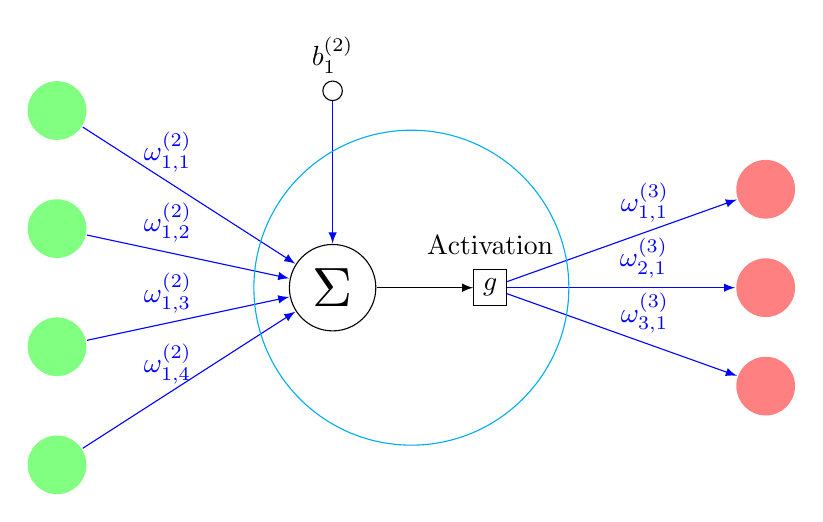
\begin{tikzpicture}[>=latex]
\path
(0,0)     node[circle,draw,scale=2,inner sep=2pt] (S) {$\Sigma$}
+(90:2.5) node[circle,draw,inner sep=2.5pt] (b) {}
          node[above=1mm] {$b_1^{(2)}$}
+(-3.5,2.25)  node[circle,scale=2.25,fill=green!50]  (x1) {} %{$T_{2m}$}
+(-3.5,0.75)  node[circle,scale=2.25,fill=green!50]  (x2) {} %{$q_v$}
+(-3.5,-0.75) node[circle,scale=2.25,fill=green!50]  (x3) {} %{$RH$}
+(-3.5,-2.25) node[circle,scale=2.25,fill=green!50]  (x4) {} %{$p_s$}
(2,0)    node[draw] (g) {$g$} node[above=3mm]{Activation}

+(3.5,1.25)  node[circle,scale=2.25,fill=red!50]  (y1) {}
+(3.5,0)  node[circle,scale=2.25,fill=red!50]  (y3) {}
+(3.5,-1.25) node[circle,scale=2.25,fill=red!50]  (y2) {};

\draw[->, black] (S)--(g);
\draw[->, blue] (b)--(S);
\draw[->, blue] (g)--(y1) node[pos=.6,above, blue]{$\omega_{1,1}^{(3)}$};
\draw[->, blue] (g)--(y2) node[pos=.6,above, blue]{$\omega_{3,1}^{(3)}$};
\draw[->, blue] (g)--(y3) node[pos=.6,above, blue]{$\omega_{2,1}^{(3)}$};

\draw[->, blue] (x1)--(S) node[pos=.4,above, blue]{$\omega_{1,1}^{(2)}$};
\draw[->, blue] (x2)--(S) node[pos=.4,above, blue]{$\omega_{1,2}^{(2)}$};
\draw[->, blue] (x3)--(S) node[pos=.4,above, blue]{$\omega_{1,3}^{(2)}$};
\draw[->, blue] (x4)--(S) node[pos=.4,above, blue]{$\omega_{1,4}^{(2)}$};
\draw[cyan] (1,0) circle(2);
\end{tikzpicture}

\caption{Computational graph showing the components participating in the activation of a neuron in the hidden layer. This example shows a 2-layer neural network with four input nodes and three output nodes. The number of nodes in the hidden layer doesn't affect the activation of the other nodes in the same layer. The sum of the weighted input and bias is passed to the activation function,
inside the hidden layers. Producing the activation of the neuron. This is again passed to the output neurons. Modified skecth based on \href{https://tex.stackexchange.com/questions/505741/architecture-neural-network-with-weights}{https://tex.stackexchange.com/questions/505741/architecture-neural-network-with-weights}. }
\label{fig:activation_one_node}
\end{figure}